\subsection{Experimental Setup and Scoring}

The tournament contained 81,216 simulations: 27,072 configurations, each repeated with three seeds. It included nine groups, households of 1, 2, 5, 9, 18, and 36 roommates, both \(u=4\) and \(u=5\), four drawer multipliers, and twelve budget and duration settings. The settings ranged from no replacement money to an unlimited budget, with durations from one to ten years. The raw file contains 578,016 roommate records and no recorded player faults. These results evaluate the tournament submission; they do not separately measure the contributions of our earlier strategies or individual components of the final strategy.

For each group present in a simulation, we first average its roommates' outcomes. Unless stated otherwise, we then give each simulation equal weight. Thus, eight copies of a group in one household do not count as eight independent experiments. Each group appears in 29,376 simulations. The supplied standings instead average individual roommate rows, giving more weight to runs with more copies of a group. Appendix~\ref{app:weighting} reports both conventions. All plots are descriptive averages over the tested settings. With only three repetitions per configuration, we do not interpret small differences as precise rankings of strategy quality.

To separate matching quality from shortages, let \(E\) be a roommate's total embarrassment and \(N_0\) its number of sockless days. We calculate
\[
E_{\mathrm{match}}=E-256^2N_0.
\]
The daily score is \(E/T\), and the mismatch component is \(E_{\mathrm{match}}/T\). We also report mismatch embarrassment per dressed day by dividing the sum of mismatch embarrassment by the sum of \(T-N_0\) across observations. This avoids treating a day without socks as successful matching. Household spending and the first day on which a replacement purchase failed are counted once per simulation. A failed purchase does not necessarily imply a subsequent sockless turn: enough socks may remain to finish the run.

\subsection{Overall Performance: Shortages Dominate the Score}

Figure~\ref{fig:overall} and Table~\ref{tab:overall} show that Group 4 was near the bottom under equal simulation weighting, with mean embarrassment of 923.63 per roommate-day. Its median was only 0.035, illustrating that most runs had very small scores while a minority incurred severe penalties. Group 4 experienced at least one sockless turn in 5.33\% of its simulations, and sockless days accounted for 99.95\% of its mean score. Preventing relatively rare availability failures would therefore have a much larger effect on this aggregate score than a comparable improvement in ordinary matching.

This does not mean our matching policy was best. Its mismatch embarrassment per dressed day was 0.689, the highest among the nine groups, compared with 0.471 for Group 8. However, the scale of these differences is small compared with the shortage penalty. Both components matter: a policy can match well while socks are available and still perform poorly over the full horizon.

\begin{figure}[htbp]
\centering
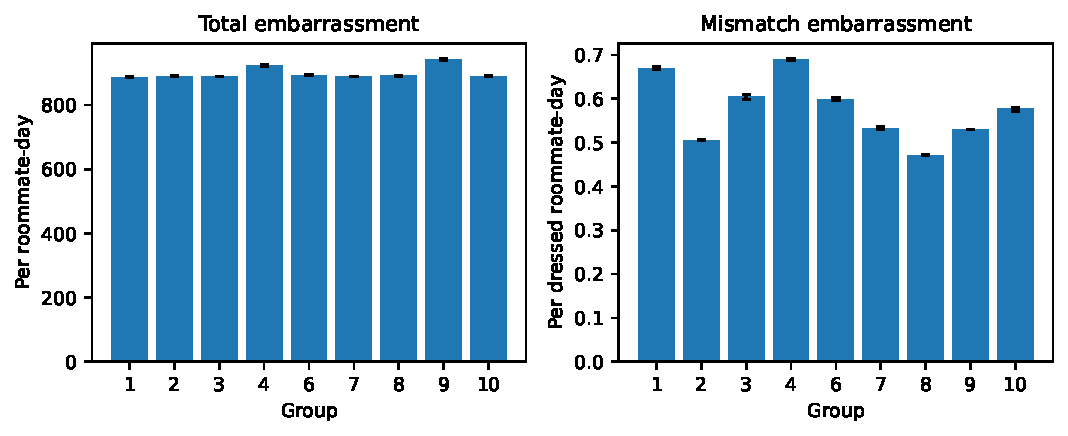
\includegraphics[width=\textwidth]{report/analysis/figures/01_overall.pdf}
\caption{Total embarrassment with equal simulation weighting (left), and mismatch embarrassment per dressed roommate-day (right). The right panel pools embarrassment and dressed days before division, so longer runs contribute more dressed days. Error bars span the three seed-specific aggregate results, not confidence intervals. Group 4 is our submission.}
\label{fig:overall}
\end{figure}

\begin{table}[htbp]
\centering
\small
\begin{tabular}{rrrrr}
\toprule
Group & Mean daily score & Median daily score & Mismatch/dressed day & Sockless runs (\%)\\
\midrule
1 & 887.33 & 0.072 & 0.670 & 5.05\\
2 & 890.14 & 0.019 & 0.506 & 5.05\\
3 & 889.05 & 0.026 & 0.605 & 5.00\\
\textbf{4} & \textbf{923.63} & \textbf{0.035} & \textbf{0.689} & \textbf{5.33}\\
6 & 893.10 & 0.025 & 0.598 & 5.14\\
7 & 889.73 & 0.011 & 0.533 & 5.33\\
8 & 891.03 & 0.021 & 0.471 & 5.22\\
9 & 941.96 & 0.028 & 0.530 & 5.57\\
10 & 890.20 & 0.026 & 0.578 & 5.07\\
\bottomrule
\end{tabular}
\caption{Each mean and median uses one average outcome per group per simulation. A sockless run has at least one sockless day for a member of that group.}
\label{tab:overall}
\end{table}
\FloatBarrier

\subsection{Budget, Duration, and Household Size}

Figure~\ref{fig:budget} restricts attention to households containing only Group 4 players. Each cell averages both draw sizes, all four drawer multipliers, and the three repetitions. Group 4 had no sockless days in any single-roommate run and averaged only 0.010 embarrassment per day in that setting. Larger households were much more vulnerable, but the household budget \(B\) was not increased with \(n\). Increasing \(n\) consequently reduced both budget per roommate-year and, at a fixed drawer multiplier and draw size, initial socks per roommate. The comparison does not isolate a cost of coordination.

Duration also matters. With nine Group 4 roommates and \(B=150\), one-year simulations averaged 0.496 embarrassment per day and had no sockless runs. Extending the same budget to two years increased the mean to 4,806.05, with sockless days in 41.7\% of runs. Even the largest finite budget, \(B=1500\), did not guarantee survival: over ten years, all 36-roommate homogeneous Group 4 runs had sockless days. Conversely, all homogeneous Group 4 runs with unlimited replacement money had zero embarrassment. The main failures therefore occurred under resource limits, although low mismatch scores under unlimited replacement do not establish that the same replacement behavior is economical.

\begin{figure}[htbp]
\centering
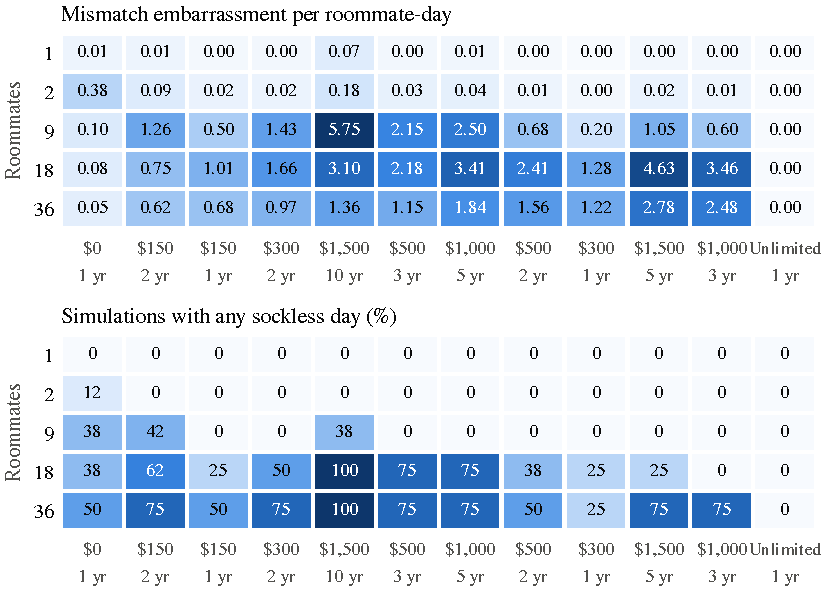
\includegraphics[width=\textwidth]{report/analysis/figures/02_budget.pdf}
\caption{Homogeneous Group 4 households. Top: mismatch embarrassment per roommate-day. Bottom: percentage of simulations with any sockless days. Columns are ordered by annual household budget, retaining the actual budget and duration. Each cell contains 24 simulations; household size changes the resources available per roommate.}
\label{fig:budget}
\end{figure}
\FloatBarrier

\subsection{Replacement Pressure and Budget Exhaustion}

Figure~\ref{fig:exhaustion} compares homogeneous households using \(\rho=10nT/(3B)\), the replacement pressure defined in Section~\ref{sec:notation}. Higher \(\rho\) means each purchased sock must support more wears. The figure includes only positive finite budgets. Outcomes at each pressure value are averaged over the compatible tested settings, so duration and initial stock still matter within this comparison.

Across all homogeneous Group 4 runs, a replacement purchase failed in 30.9\%, whereas sockless days occurred in 22.8\%. In 8.1\% of runs, purchases failed but the remaining drawer lasted through the horizon. Exhaustion is therefore a useful warning rather than an interchangeable measure of failure. Its timing matters as well: an early failed purchase leaves more time for holes and discards to deplete the remaining stock. The high-pressure portion of Figure~\ref{fig:exhaustion} shows earlier purchase failures and a larger fraction of sockless days. Other groups also struggled in this region, indicating that some tested budgets were broadly difficult, while Group 4's additional losses show that its safeguards did not fully control this risk.

\begin{figure}[htbp]
\centering
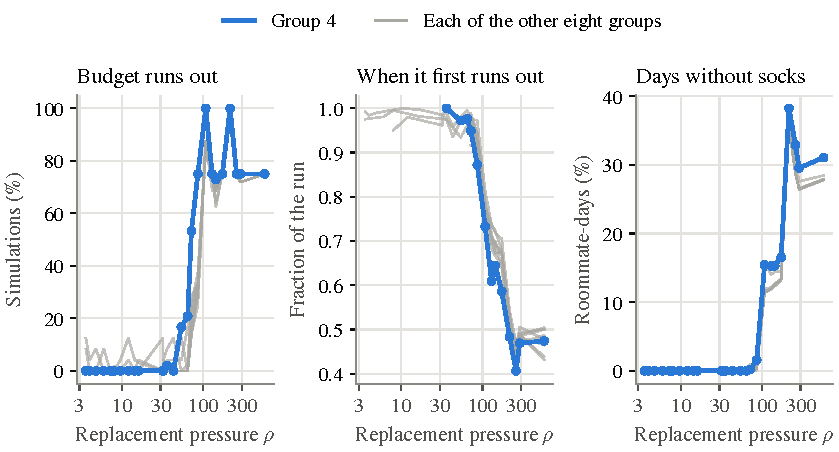
\includegraphics[width=\textwidth]{report/analysis/figures/03_exhaustion.pdf}
\caption{Positive finite budgets in homogeneous households. The panels show the frequency of failed replacement purchases, their average timing conditional on failure, and the percentage of roommate-days without socks. The comparison line is the median of the eight other groups' averages at each \(\rho\). The horizontal axis is logarithmic; connected points summarize tested settings rather than a fitted response curve.}
\label{fig:exhaustion}
\end{figure}
\FloatBarrier

\subsection{The Influence of Other Roommates}

Figure~\ref{fig:neighbors} compares Group 4 with each other group under the same budget, duration, draw-size, and drawer-multiplier grid. In two-person households, its mean score ranged from 30.40 with Group 2 to 63.91 with Group 10. Yet every partner produced the same 1.04\% frequency of runs with Group 4 sockless days. Differences in total score can therefore reflect the severity and duration of shortages, even when their frequency is unchanged.

In nine-person households, a single Group 4 player among eight Group 9 players averaged 1,223.54 embarrassment per day, compared with 991.84 among eight Group 3 players. When eight players used Group 4 and only one used another policy, Group 4 averaged 1,353.56 with a Group 9 neighbor. These results show sensitivity to household composition, but the best neighbor depends on the metric: among eight Group 7 players, Group 4's mismatch component was only 0.418 per day, compared with 1.215 among eight Group 1 players. A neighbor that supports close matching need not minimize shortage risk.

The raw file records household spending, not individual discard decisions or individual expenditure. We therefore cannot identify which roommate caused a particular purchase failure. Appendix~\ref{app:externalities} extends this comparison to changes in the outcomes of other groups when Group 4 enters a five-person household.

\begin{figure}[htbp]
\centering
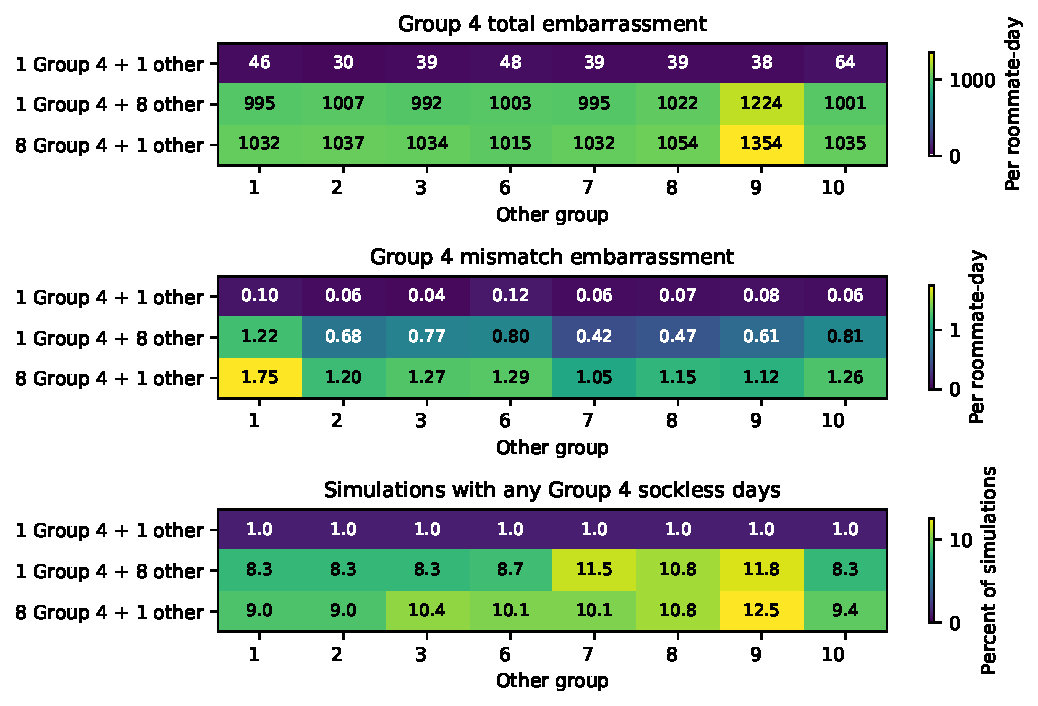
\includegraphics[width=\textwidth]{report/analysis/figures/04_neighbors.pdf}
\caption{Group 4 outcomes by the other group and Group 4's role in the household. Each cell averages 288 simulations covering the same resource grid. In the majority case, scores first average the eight Group 4 players within a simulation; a sockless run requires at least one of those players to go without socks.}
\label{fig:neighbors}
\end{figure}
\FloatBarrier

\subsection{Initial Drawer Capacity Can Delay or Prevent Shortages}

Figure~\ref{fig:capacity} varies drawer capacity within fixed household types and budget-duration settings. For 36 Group 4 roommates with \(B=300\) over one year, doubling the base drawer reduced mean embarrassment from 12,898.96 to 1.85 and eliminated sockless days in the tested runs. Initial capacity can consequently determine whether a household survives a short horizon even when replacement money per roommate is small.

The protection was incomplete over longer horizons. With 36 Group 4 roommates and \(B=1500\) over ten years, increasing the drawer multiplier from 1 to 10 reduced sockless roommate-days from 73.0\% to 36.5\%, but did not remove shortages. A large initial drawer is a finite buffer, so its contribution becomes smaller relative to total wear as \(T\) grows. The mixed 36-person households showed a similar pattern.

More capacity also did not improve ordinary matching monotonically. In nine-person homogeneous households with \(B=300\) over one year, there were no sockless days at any drawer multiplier, but daily embarrassment increased from 0.139 at multiplier 1 to 0.373 at multiplier 2 before falling to 0.041 at multiplier 10. Capacity changes the evolving shade distribution as well as the available stock; the aggregate records cannot determine the exact mechanism behind this pattern.

\begin{figure}[htbp]
\centering
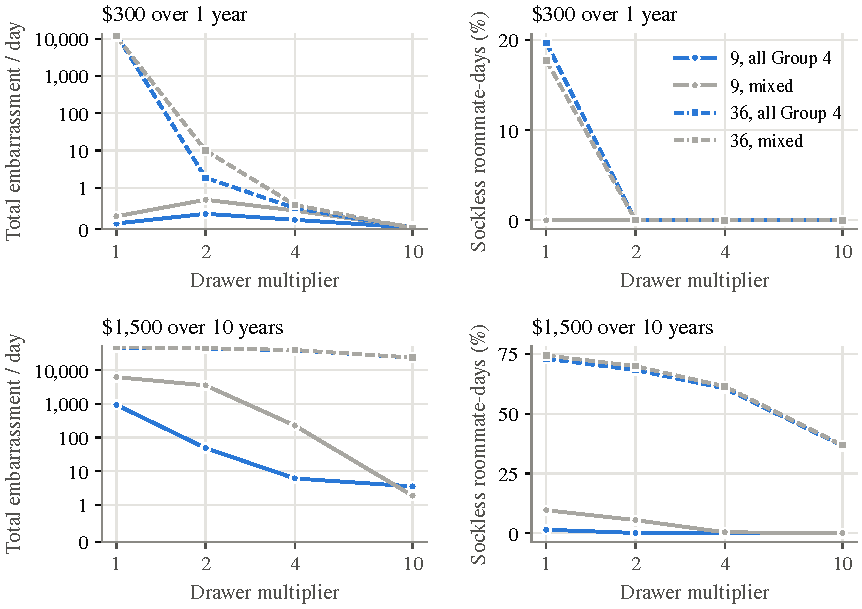
\includegraphics[width=\textwidth]{report/analysis/figures/05_capacity.pdf}
\caption{Group 4 in homogeneous and mixed households of 9 and 36 roommates, holding budget and duration fixed within each row. Each point averages both draw sizes and three repetitions. Mixed households contain one or four players from each group, respectively. Total-score axes are logarithmic above 1 and linear near zero; sockless percentages use linear axes.}
\label{fig:capacity}
\end{figure}
\FloatBarrier

\subsection{Drawing Four Versus Five Socks}

We matched the \(u=4\) and \(u=5\) runs by roster, budget, duration, drawer multiplier, and seed, giving 14,688 paired comparisons for Group 4. Figure~\ref{fig:unit} shows an improvement at every household size. Across these pairs, mean daily embarrassment fell from 1,071.10 to 776.16, a reduction of 27.5\%. The mismatch component fell from 0.751 to 0.084 per roommate-day, and sockless roommate-days fell from 1.63\% to 1.18\%. Thus, the improvement included both better matching and greater availability.

These comparisons evaluate the tested five-sock setup as a whole. Its base drawer was also larger: for example, with nine roommates it contained 60 socks instead of 48, and with 36 roommates it contained 192 instead of 156. There were no paired runs holding the actual drawer capacity \(C\) constant while changing \(u\). The extra candidate sock increases the number of possible pairs from six to ten, but these data cannot separate that advantage from the benefit of the larger drawer.

\begin{figure}[htbp]
\centering
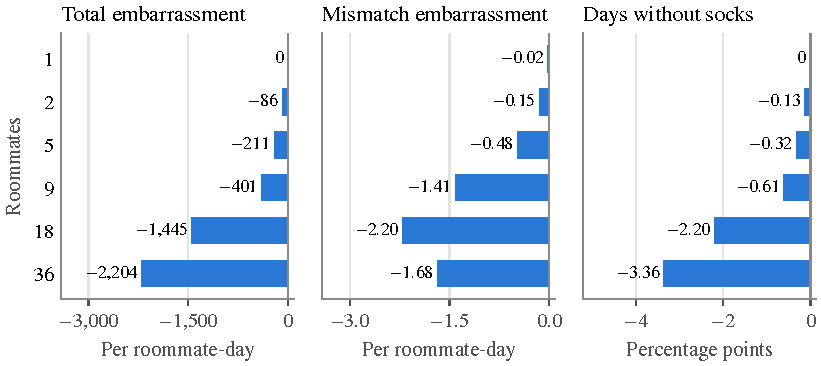
\includegraphics[width=\textwidth]{report/analysis/figures/06_unit.pdf}
\caption{Mean paired changes for Group 4 from the four-sock to the five-sock setup, grouped by household size. Negative values indicate improvements. Each comparison holds roster, budget, duration, drawer multiplier, and seed fixed, but actual drawer capacity increases with draw size.}
\label{fig:unit}
\end{figure}
\FloatBarrier
